\chapter{Introduzione}
Il sito web www.dell.it non � altro che la trasposizione italiana del sito internet www.dell.com, portale informatico dell'omonima casa produttrice di personal computer. Tale sistema si propone, sia come vetrina/negozio per soluzioni notebook e desktop, per accessori per pc, materiale elettronico di varia natura, come ad esempio televisori, sistemi home theater, sia come portale per accedere al supporto per i prodotti sopra citati venduti dall'azienda. Le soluzioni offerte dalla Dell Inc. riguardano sia i clienti privati con un ``Business to Consumer'' che i clienti aziendali offrendo un ``Business to Business''.\\
Quello che si propone la Dell Inc. con questo sito web, � di avere un contatto diretto con i propri clienti, eliminando le grandi catene di distribuzione e intermediari. Tale soluzione le consente di avere prezzi pi� concorrenziali, offrire la possibilit� di ``personalizzare'' molti prodotti e di garantire servizi post-vendita che fidelizzino il cliente alla societ� texana.\\
Per garantire questo tipo di commercio la Dell Inc, ha puntato molto sull' e-business, categoria nella quale possiamo collocare il sito web preso in esame. Il commercio elettronico, come una qualsiasi altra transazione economica si fonda su diverse fasi:
\begin{itemize}
\item La transazione economica si compone di una fase di ricerca, in cui il cliente cerca sul mercato i fornitori potenzialmente in grado di soddisfare i suoi requisiti
\item {\it Negoziazione}: il cliente interagisce con i fornitori individuati per vericare se e a quali condizioni possono essere soddisfatti i propri requisiti. Questa fase si conclude con la scelta del fornitore e del prodotto
\item {\it Esecuzione}: il bene scelto in precedenza viene consegnato al cliente
\item Controllo, ha l'obiettivo di gestire eventuali eccezioni che possono vericarsi (per esempio, la fornitura al cliente di un bene difettoso).
\end{itemize}
Nel caso della Dell Inc. tutte queste fasi sono state automatizzate e informatizzate, pertanto il possedere uno strumento informatico facile da gestire e funzionale per i clienti diventa di fondamentale importanza per il business dell'azienda. Lo scopo di tale relazione � verificare l'usabilit� della versione italiana di tale portale web.\\
Nel primo capitolo presenteremo il sito web in questione e successivamente  forniremo la pianificazione dell'attivit� svolta e definiremo il profilo utente.

\section{Descrizione del sistema}
Il portale preso in esame, {\it www.dell.it}, appartiene alla categoria dei Web System Information del tipo e-commerce e informativo: consente di scegliere e acquistare una vasta gamma di prodotti high tech, mentre dal punto di vista informativo si possono apprendere svariate notizie riguardanti l'azienda, dalla storia della Dell Inc., alle politiche ambientali adottate dal'azienda.\\
\begin{figure}[!h]
\centering
\includegraphics[scale=0.75]{figure/home_page.eps}
\caption{Home page del sito web www.dell.it} \label{fig:home_page}
\end{figure}\\
L'home page, come mostrata in figura\ref{fig:home_page}, pu� essere suddivisa in tre macroaree e in una intestazione a pi� pagina. Scorrendo la pagina dall'alto verso il fondo troviamo:
\begin{enumerate}
\item Un primo men� orizzontale che consente di accedere rapidamente alle pagine informative suddivise per clientela (privati, piccole-medie imprese, pubblica amministrazione, grandi imprese) e a fianco un piccolo men� per richiedere assistenza o effettuare il login. Sulla sinistra � sempre presente il logo dell'azienda che, oltre allo scopo pubblicitario, ha anche la funzione di rimandare l'utente alla home page.
\item Nella parte centrale � stato riservato un ampio spazio alla vetrina dei prodotti maggiormente pubblicizzati, offerte speciali. Sono perlopi� immagini a ciclo continuo che occupano l'intera area. Anche tali immagini sono dei link che rimandano al prodotto visualizzato in quel momento.
\item A fondo pagina troviamo un secondo men� orizzontale che riporta ulteriori link alle aree descritte al punto 1. Troviamo inoltre anche aree dedicate all'account personale dell'utente, al supporto e alle informazioni sulla societ�.
\end{enumerate}
Come � chiaramente visibile, il portale web � assai esteso sia in ampiezza, con un buon numero di sezioni, sia in profondit�, con un ampio numero di livelli e sotto livelli che appartengono ad ogni sezione; pertanto si � stabilito di concentrare e limitare la valutazione alla sezione a noi pi� affine, ossia alla sezione {\it PER LA CASA}, denominazione che � stata data per la categoria degli utenti privati, ossia persone che non hanno la possibilit� di scaricare l'IVA, e hanno richieste assai differenti dalle aziende: ad esempio il fattore di personalizzazione per i privati � molto elevato (si va dall'aspetto estetico fino ai componenti dell'intero computer) ed � presente su molteplici modelli; per i clienti aziendali questo aspetto � molto limitato se non addirittura assente.\\
La figura \ref{fig:home_privati1} mostra la pagina con la quale un utente privato si trover� a interagire fin dall'inizio, e con la quale potr� iniziare la navigazione per ottenere ci� che desidera, sia che sia un un ``acquisto'' o che sia del ``supporto''. Di default il sistema mostra la sezione ``acquisti''. Presenteremo queste due parti oltre alla home page, poich� sono le due pagine web con le quali l'utente dovr� interagire maggiormente, pertanto sono di fondamentale importanza per una buona navigabilit� e usabilit�.\\
Analizzando nel dettaglio la pagina caricata di deafult, troviamo che � divisa anch'essa in tre parti: l'intestazione composta da una serie di titoli che consentono di accedere a tutte le varie categorie di prodotti offerti. Ogni categoria (offerti speciali, Notebook \& Mini, etc...) apre un men� a discesa che consente di scegliere una determinata categoria di modelli. 
\begin{figure}[!h]
\centering
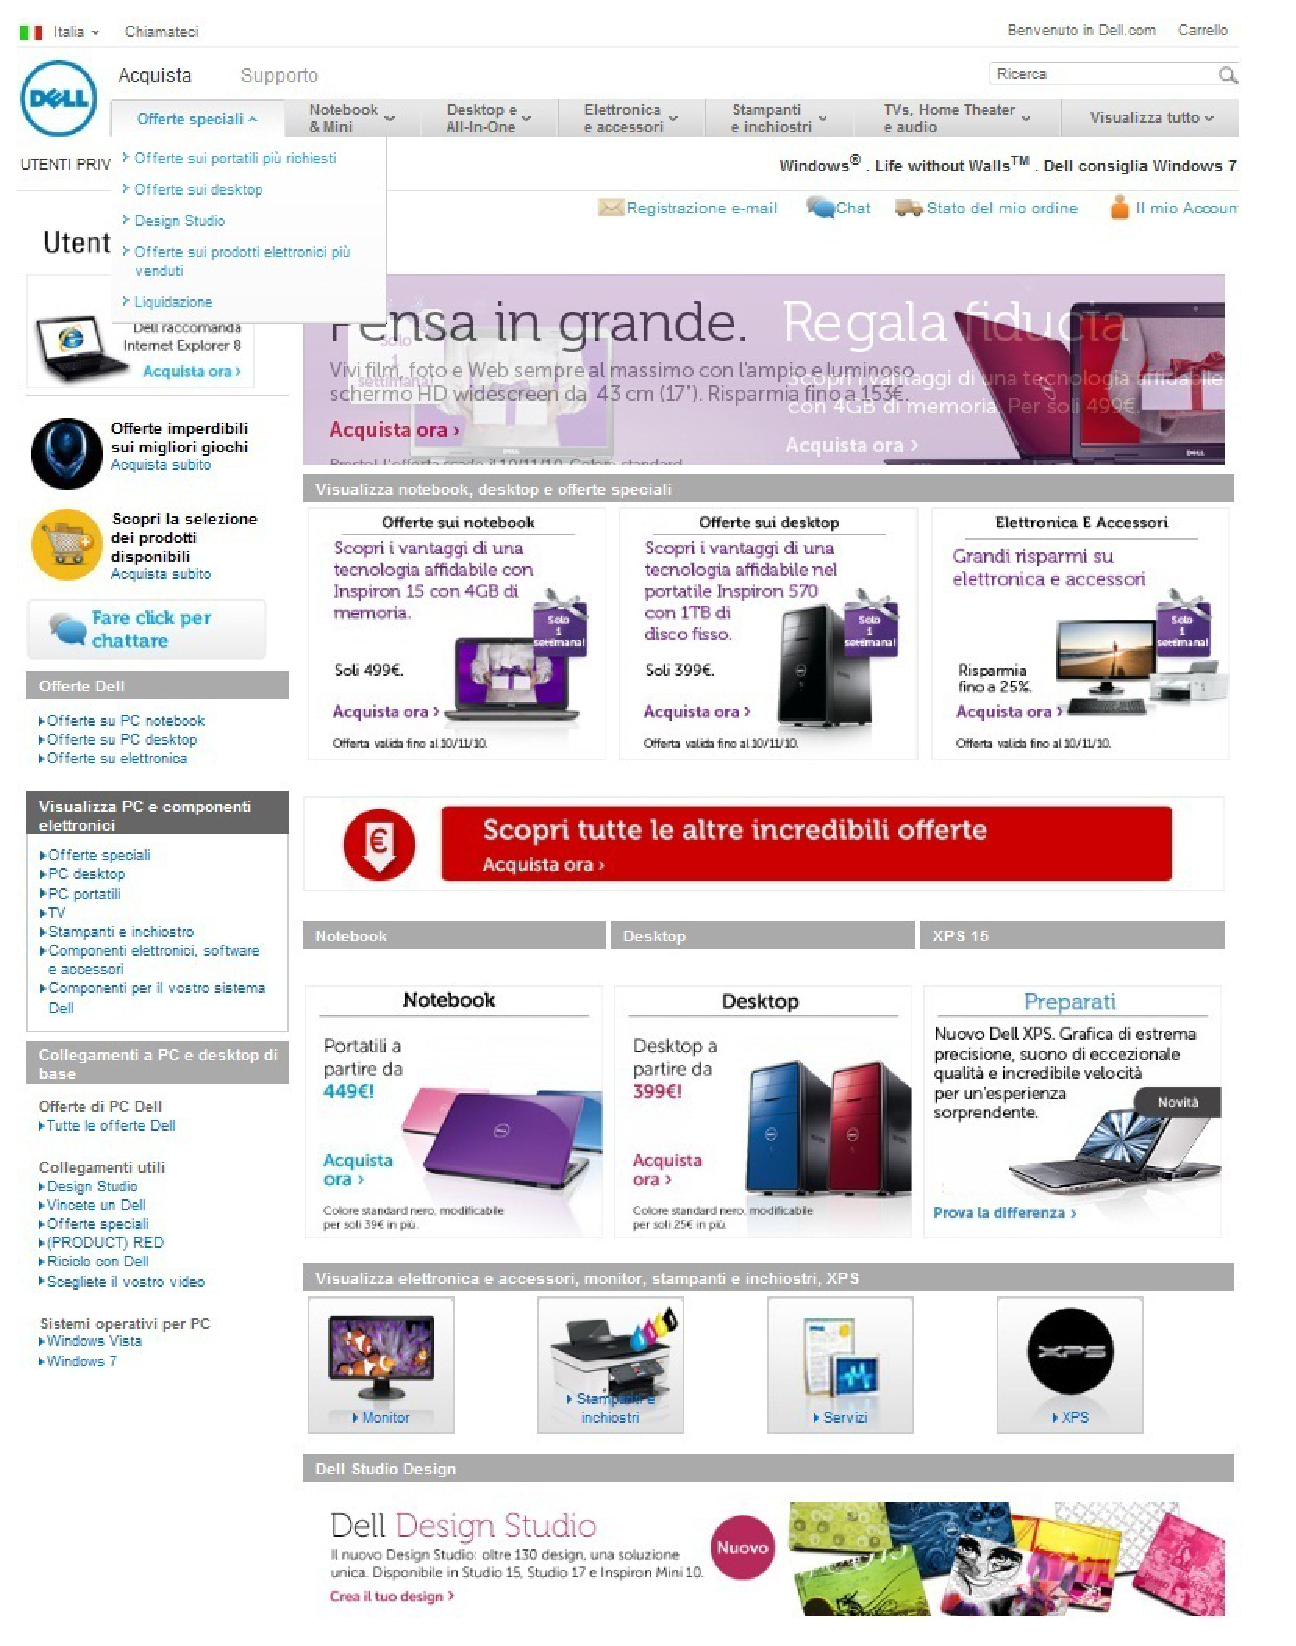
\includegraphics[scale=0.73]{figure/privati1.eps}
\caption{Home page sezione ``Per la casa''. Si pu� notare il men� a discesa della sezione ``Offerte speciali''} \label{fig:home_privati1}
\end{figure}\\
\newpage
Le sezioni raggiungibili da tramite questo men� sono:
\begin{itemize}
\item {\bf Offerte speciali}: racchiude una serie di link diretti che conducono alle offerte sulle varie categorie di prodotti. Tali offerte possono essere relative a prodotti che oramai la Dell non ha pi� intenzione di produrre oppure prodotti maggiormente venduti che sono associati a un qualche genere di promozione.
\item {\bf Notebook \& Mini}: racchiude tutte le categorie di notebook e pc mini che la Dell Inc. produce. Troviamo in testa due collegamenti alle offerte e ai prodotti in liquidazione a cui succedono vari link che visualizzano i diversi prodotti: prima il nome della famiglia in azzurro chiaro e appena sotto in grigio tutti i modelli che appartengono a tale famiglia; vengono mostrati all'utente in ordine crescente di prestazioni, mentre a fondo men�, separato da una linea troviamo link d'utilit� come il confronto tra prodotti diversi.
\item {\bf Desktop e All-in-One}: Come per la famiglia dei portatili lo schema di visualizzazione rimane lo stesso: il collegamento alle offerte e liquidazione, successivamente le varie soluzioni desktop e All-in-One, con la suddivisione famiglia-modello, sempre mostrate in ordine crescente di prestazioni e in fondo al men� i link d'utilit� per il confronto e l'accesso diretto agli accessori
\item {\bf Elettronica e accessori}: tale men� permette di accedere a un insieme di prodotti molto eterogeneo: dai lettori mp3 agli accessori per notebook e desktop. In tale men� la visualizzazione non prevede che per ogni categoria vengano elencati anche tutti i nomi dei prodotti, ma solamente la categoria a cui appartengono (Mp3, GPS, etc...)
\item {\bf Stampanti e inchiostri}: racchiude tutte le stampanti che possono essere acquistate tramite il sito internet. Lo schema di visualizzazione � lo stesso usato per la sezione ``Elettronica e accessori'': vengono mostrate solamente le varie famiglie di prodotti senza elencare i singoli modelli
\item {\bf TVs, Home Theater e audio}: permette di accedere alle pagine in cui vengono mostrati le soluzione per l'intrattenimento domestico, con tv di varia grandezza, soluzioni audio e video. Lo schema di visualizzazione � lo stesso degli ultimi due men�
\item {\bf Visualizza tutto}: apre un men� in cui compaiono tutti le categorie di prodotti precedentemente citati: un'intestazione in azzurro chiaro per la categoria (stessa dicitura precedentemente) e in grigio le varie famiglie che appartengono a tale categoria
\end{itemize}
Tornando ad esplorare la pagina (fig:\ref{fig:home_privati1}) troviamo una colonna posta sulla sinistra composta da una serie di link a pagine appartenenti alle sezioni alle quali si pu� accedere anche dai men� precedentemente citati; questo elenco riporta per la maggior parte link di maggior interesse, sono prevalentamente le pagine pi� richieste dall'utente. La restante parte della pagina � dedicata a una serie d'immagini, tutte con funzione di link, che riportano pubblicit� di offerte, nuovi prodotti, o comunque soluzioni che l'azienda vuole mettere in maggior risalto. A fondo della schermata troviamo un secondo men� riassuntivo comprendente tutta una serie di collegamenti che consentono all'utente di accedere alle sezioni prima elencate e in aggiunta anche alle sezioni riguardanti l'azienda, informazioni personali e condizioni d'uso. In ultimo vi � un trafiletto sulle offerte e condizioni generali sull'utilizzo del sito web (fig:\ref{fig:home_privati2}).
Come la maggior parte dei siti web di e-commerce fanno uso della metafora {\it carrello} per indicare tutti quei prodotti scelti dall'utente, configurati e pronti per essere acquistati, ma non ancora confermati definitivamente;nel nostro caso � presente un link diretto a tale elenco ed � sempre posto, in tutte le pagine della sezione ``acquisti'', in alto a destra.
\begin{figure}[!h]
\centering
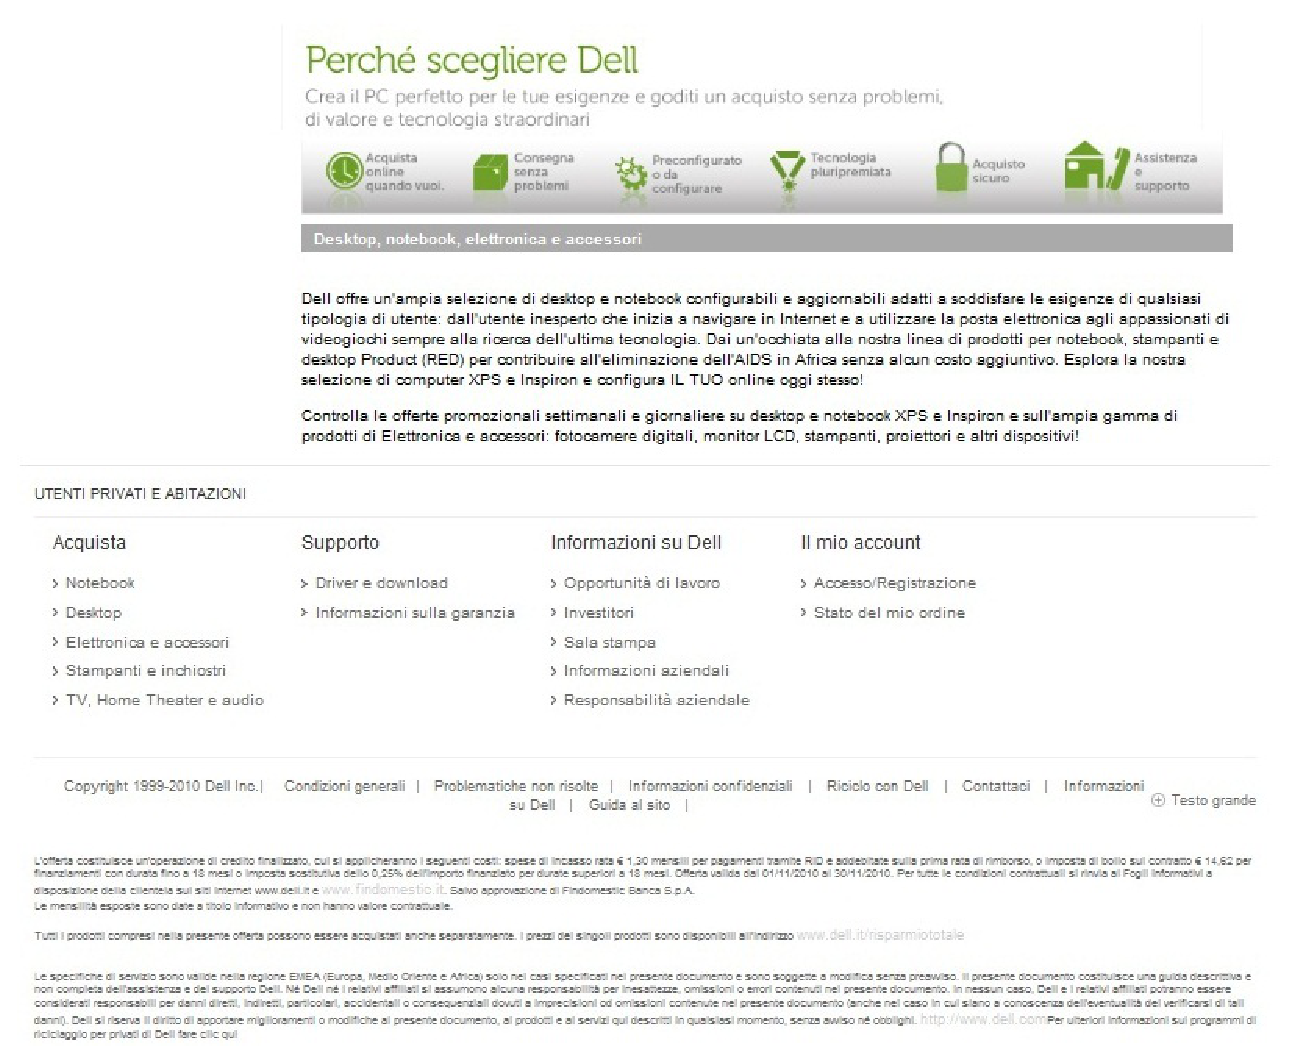
\includegraphics[scale=0.75]{figure/privati2.eps}
\caption{Fondo pagina della sezione ``Per la casa'' sezione ``Acquisti''} \label{fig:home_privati2}
\end{figure}\\
\newpage
Il passaggio alla sezione supporto � reso possibile dal posto in alto a sinistra con la scritta ``Supporto''. Nella pagina visualizzata troviamo che lo schema di  � lo stesso di quello usato per la sezione ``acquisti'': una barra orizzontale che mostra diverse utilit� di carattere generico (campo di ricerca,link al login,un link diretto alla home page, etc...), e in aggiunta un men� orizzontale che consente di accedere alle vere e propri categorie di supporto. Tali sezioni sono:
\begin{itemize}
\item {\bf Driver e download}: consente di scaricare varie tipologie di driver per accessori e prodotti Dell. Fornisce inoltre aiuto nel caso l'utente abbia problematiche a installare un sistema operativo differente su un prodotto Dell.
\item {\bf Assistenza per il prodotto}: fornisce manuali d'uso, risoluzione delle problematiche pi� comuni, aggiornamenti e supporto per il ritiro dei prodotti
\item {\bf Supporto per argomento}: le problematiche sono trattate per argomento; � da sottolineare che tali argomenti sono in massima parte argomenti di tipo software, specialmente sui vari sistemi operativi forniti all'acquisto di un computer, pertanto si trovano esclusivamente sistemi operativi Microsoft. Possiamo trovare anche aiuti sulla configurazione delle reti wireless o sulla sicurezza
\item {\bf Assistenza per l'ordine}: viene trattato tutto ci� che riguarda l'ordine di un utente: lo stato di avanzamento, la restituzione del prodotto, le segnalazioni di danneggiamento o di malfunzionamenti dello stesso
\item {\bf Informazioni sulla garanzia}: vengono date note informative sui termini legali della garanzia e delle varie estensioni proposte dalla Dell Inc. e accedere a particolari tipi di assistenza
\item {\bf Visualizza tutto}: come nel caso della precendente (sezione ``acquisti'') anche in questo caso tale dicitura consente di visualizzare un sommario di tutte le voce appena descritte, suddividendole in categorie come nel men� ed elenco le sottovoci del men� a discesa
\end{itemize}
Tornando ad analizzare la pagina nel suo complesso possiamo ritrovare a sinistra un elenco di link che riprendono ci� che possiamo trovare nel men� precedentemente descritto, suddivisi nelle medesime sezioni, mentre nella sezione centrale della pagina un ricco assortimento di icone e ulteriori link alle varie sezioni di supporto all'utente. Da tali icone si pu� accedere alle aree dedicate alla community e ai contatti diretti con gli operatori. 
A fondo pagina � riportato il medesimo schema della sezione acquisti con un elenco di tutte le categorie e delle condizioni generali d'utilizzo del portale.
\begin{figure}[!h]
\centering
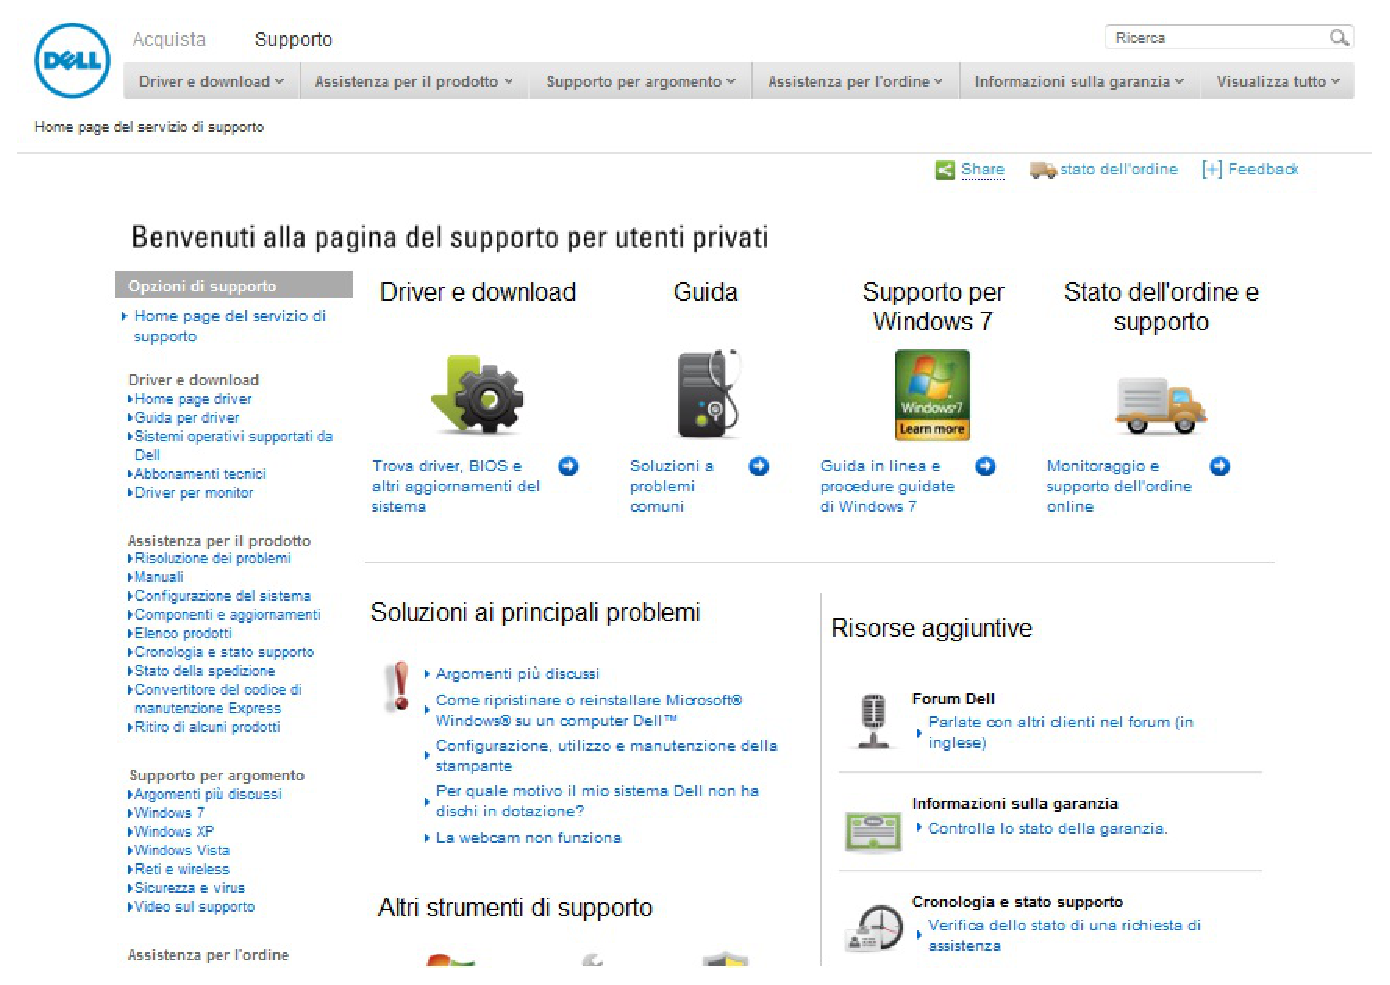
\includegraphics[scale=0.7]{figure/supporto1.eps}
\caption{Home page sezione ``Per la casa''. Si pu� notare il men� a discesa della sezione ``Offerte speciali''} \label{fig:supporto}
\end{figure}\\


\section{Pianificazione del lavoro}
La prima riunione del gruppo � avvenuta il giorno 13 luglio presso la facolt� d'ingegneria di Brescia. Calendario alla mano abbiamo iniziato a pianificare l'attivit� di valutazione del sito web scelto; valutando l'ampia disponibilit� di tempo libero nella pausa estiva e considerando i vari impegni sia personali che universitari, abbiamo ritenuto plausibile di completare il lavoro per la sessione d'esame di dicembre/gennaio. Non era stata stabilit� una data precisa in quanto non era ancora stata fissata alcuna data d'esame per tale periodo.\\
Una volta definita una simbolica data di terminazione, stabilita per l'8 dicembre abbiamo iniziato il lavoro di pianificazione dell'attivit�, avvalendoci come strumento di aiuto, del diagramma di Grantt abbiamo cercato di pianificare tutte le fasi del progetto.\\
\newline
\begin{figure}[!h]
\centering
\includegraphics[angle=90,scale=0.52]{figure/grantt.eps}
\caption{Grafico di Grantt per la pianificazione del lavoro}
\label{fig:grantt}
\end{figure}
A causa d'impegni imprevisti sia di carettere universitario che lavorativo, il diagramma di Grantt mostrato in figura \ref{fig:grantt} � rimasto una mera idea, e tutte le tempistiche hanno subito grossi ritardi e slittamenti, anche di parecchie settimane; tali ritardi sono da imputare a guasti imprevisti, esami e impegni di lavoro. In particolare le fasi ``Debriefing'' dopo l'esperimento con gli utenti e le ``Proposte di soluzioni'' hanno subito i maggiori ritardi. La stesura della relazione ha richiesto pi� tempo di quanto preventivato, in quanto gli impegni dei membri del gruppo non consentivano di avere dei summit regolari, per verificare l'effettivo stato di avanzamento del progetto. 

\section{Definizione del profilo utente}
Scopo del presente paragrafo � delineare gli attributi di un probabile utente
utilizzatore del sistema in esame. Questa � una fase cruciale di ogni analisi di usabilit�, infatti le assunzioni qui prese condizioneranno i successivi metodi di valutazione.\\
Avvalendoci del nostro buon senso, abbiamo stilato un profilo psicologico dell'utente medio che accede al sito web; � stato valutato e consultato il forum di supporto, tuttavia essendo rivolto esclusivamente a coloro che hanno dei problemi, non ci d� informazioni utili: coloro che discutono nel forum sono persone generalmente abituate a una forte autonomia, mentre utenti novizi, a fronte di un problema � pi� facile che cerchino l'aiuto di una persona esperta, come un amico, il quale poi successivamente chieder� aiuto sul forum.\\
In base a tale ragionamento abbiamo provato a stilare un elenco di caratteristiche che delineano la classe di utenti/clienti del portale:\\

\smallskip

{\bf \noindent Caratteristiche Psicologiche}
\begin{itemize}
\item Stile cognitivo: il sistema permette a chi ha delle conoscenze pregresse di sfruttarle, mentre coloro che sono meno esperti vengono supportati dal sistema: mostra le procedure sempre uguali e, per persone che sono pi� intuitive, il sito web fornisce alternative al percorso tradizionale
\item Attitudine (dell'utente rispetto al sistema): positiva, gi� il fatto che
l'utente tenti di comprare via internet indica che � ben disposto
all'utilizzo del sito. Ovviamente avendo il sito web anche la funzione di vetrina, risulta essere adatto anche a coloro che vogliono solamente farsi un'idea delle soluzioni informatiche presenti sul mercato 
\item Motivazione (dell'utente rispetto all'uso): alta, in quanto non � possibile acquistare in un negozio tradizionali i prodotti Dell
\end{itemize}

{\bf \noindent Conoscenze}
\begin{itemize}
\item Livelli di alfabetizzazione (lettura): l'utente deve saper leggere e comprendere le istruzioni che gli vengono visualizzate sullo schermo
\item Titolo di studio: minimo, licenza media
\item Abilit� dattilografica: bassa, in quanto l'interazione con il portale necessita in larga parte dell'utilizo del mouse, mentre la tastiera � utilizzata solo per funzionalit� specifiche e molto limite
\item Linguaggio: in massima parte il sito web risulta essere tradotto in molteplici lingue di tutto il mondo, anche se verr� specificato nei capitoli successivi, vi sono ancora determinate parti rimaste in inglese
\item Alfabetizzazione informatica: moderata, l'utente � capace di navi-
gare su internet, quindi, conosce i rudimenti dell'informatica. Inoltre per certe funzionalit� deve saper riconoscere alcuni componenti di un computer, ma non � un requisito fondamentale
\end{itemize}
{\bf \noindent Esperienza}
\begin{itemize}
\item Uso dei sistemi informatici: media, in quanto l'utente deve saper navigare nel web e deve avere un'esperienza positiva con il pagamento tramite carte di credito o prepagata. Un utente novizio, con scarsa esperienza nell'utilizzo di tali strumenti potrebbe avere dei dubbi sulla sicurezza della metodologia di pagamento e sull'affidabilit� dei corrieri
\item Dell'applicazione: nessuna, in quanto il sito internet si propone con finestre intuitive che consentono anche ad utenti meno esperti di poter usufriuire del portale con successo 
\end{itemize}
{\bf \noindent Caratteristiche fisiche dell'utente}
\begin{itemize}
\item Vista: requisito fondamentale � che l'utente non sia cieco, in quanto il sistema non prevede una navigazione per non i vedenti (non rispetta gli standard del W3C. Per quanto riguarda il resto dei difetti, non vi sono problemi, poich� un eventuale daltonismo non comporta alcun tipo di limitazione
\item Manualit�: non vi � nessun vincolo, basta poter usare la tastiera  il mouse, o periferiche sostitutive alle due citate
\item Maggioreit�: per poter effettuare un ordine valido � necessario essere maggiorenni, in quanto il pagamento elettronico o il bonifico bancario richiedono tale caratteristica; da sottolineare che la registrazione al sito della Dell, non effettua alcun tipo di controllo sull'et�, pertanto si potrebbe ordinare un prodotto anche senza essere maggiorenni
\end{itemize}
{\bf \noindent Caratteristiche sociali}
\begin{itemize}
\item Tipologia di lavoro: nessun requisito, poich� per acquistare basta essere maggiorenni
\item Frequenza di turn-over: alta, in quanto quasi sempre nuovi gli utenti che acquistano, vista anche la durabilit� del bene acquistato
\item Importanza del compito: bassa in genere, serve solo per soddisfare un bisogno dell'utente; se viene incluso l'accesso alla sezione del supporto allora la frequenza del turno over pu� essere considerata moderata.
\item Frequenza d'uso: estremamente bassa, poich� salvo ulteriori acquisti o la necessit� di richiedere assistenza, l'utente potrebbe anche non aver pi� bisogno di usare il portale
\item Addestramento di base: nessuno, il sito dovrebbe essere autoesplicativo
\end{itemize}
Dall'analisi appena effettuata possiamo dire che la popolazione d'utenti utlizzatori del sito � altamente variagata, se poi si pensa che il sito web si compone anche delle sezioni per le aziende e per la pubblica ammistrazione, la variet� di tipologie d'utenti aumenta notevolmente, considerando aspetti pi� professionali e meno legati al puro svago.\\
Nei capitoli che seguono abbiamo utilizzato il profilo appena tracciato per effettuare la valutazione.

